\documentclass[ reprint, amsmath,amssymb, aps,prx]{revtex4-2}
\usepackage{amsmath}
\usepackage{amssymb}
\usepackage[usenames,dvipsnames]{xcolor}
\usepackage[colorlinks=true,citecolor=blue,linkcolor=blue]{hyperref}
\usepackage{tikz}

\begin{document}

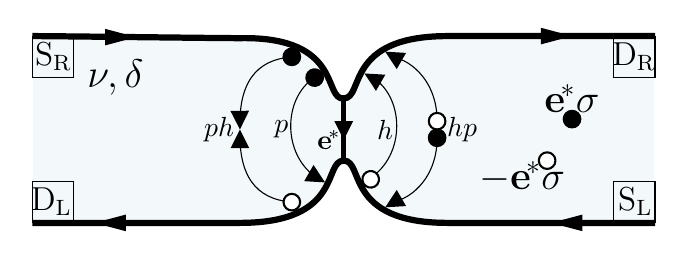
\begin{tikzpicture}[x=0.75pt,y=0.75pt,yscale=-1,xscale=1]
\draw  [color={rgb, 255:red, 255; green, 255; blue, 255 }  ,draw opacity=1 ][fill={rgb, 255:red, 173; green, 216; blue, 230 }  ,fill opacity=0.15 ] (100,110) -- (400,110) -- (400,200) -- (100,200) -- cycle ;
\draw [fill={rgb, 255:red, 255; green, 255; blue, 255 } ,fill opacity=1 ][line width=2.25]    (100,110) .. controls (110,110) and (190,111) .. (200,111) .. controls (250,110) and (240,141) .. (250,140) .. controls (260,140) and (250,110) .. (300,110) .. controls (310,110) and (390,110) .. (400,110) ;
\draw [shift={(360,110)}, rotate = 180] [fill={rgb, 255:red, 0; green, 0; blue, 0 }  ][line width=0.08]  [draw opacity=0] (15,-4) -- (0,0) -- (15,4) -- cycle    ;
\draw [shift={(150,110.5)}, rotate = 180] [fill={rgb, 255:red, 0; green, 0; blue, 0 }  ][line width=0.08]  [draw opacity=0] (15,-4) -- (0,0) -- (15,4) -- cycle    ;
\draw [fill={rgb, 255:red, 255; green, 255; blue, 255 }  ,fill opacity=1 ][line width=2.25]    (400,200) .. controls (390,200) and (310,200) .. (300,200) .. controls (250,200) and (260,170) .. (250,170) .. controls (240,170) and (250,200) .. (200,200) .. controls (190,200) and (110,200) .. (100,200) ;
\draw [shift={(130,200)}, rotate = 0] [fill={rgb, 255:red, 0; green, 0; blue, 0 }  ][line width=0.08]  [draw opacity=0] (15,-4) -- (0,0) -- (15,4) -- cycle    ;
\draw [shift={(350,200)}, rotate = 0] [fill={rgb, 255:red, 0; green, 0; blue, 0 }  ][line width=0.08]  [draw opacity=0] (15,-4) -- (0,0) -- (15,4) -- cycle    ;
\draw    (236,130) .. controls (220,140) and (220,170) .. (240,180) ;
\draw [shift={(241,180.5)}, rotate = 210] [fill={rgb, 255:red, 0; green, 0; blue, 0 }  ][line width=0.08]  [draw opacity=0] (9,-4.5) -- (0,0) -- (9,4.5) -- cycle    ;
\draw [shift={(236,130)}, rotate = 150] [color={rgb, 255:red, 0; green, 0; blue, 0 }  ][fill={rgb, 255:red, 0; green, 0; blue, 0 }  ][line width=0.75]      (0, 0) circle [x radius= 4, y radius= 4]   ;
\draw (220,155) node   {$p$};
\draw    (264,130) .. controls (280,140) and (280,170) .. (260,180) ;
\draw [shift={(263,179)}, rotate = 150] [fill={rgb, 255:red, 255; green, 255; blue, 255 }  ][line width=0.75]      (0, 0) circle [x radius= 4, y radius= 4]   ;
\draw [shift={(260,128)}, rotate = 30] [fill={rgb, 255:red, 0; green, 0; blue, 0 }  ][line width=0.08]  [draw opacity=0] (9,-4.5) -- (0,0) -- (9,4.5) -- cycle    ;
% Text Node
\draw (270,155) node  [font=\normalsize]  {$h$};
\draw    (272,120) .. controls (280,120) and (295,130) .. (295,151) ;
\draw [shift={(295,151)}, rotate = 90] [fill={rgb, 255:red, 255; green, 255; blue, 255 }  ][line width=0.75]      (0, 0) circle [x radius= 4, y radius= 4]   ;
\draw [shift={(270,117.5)}, rotate = 30] [fill={rgb, 255:red, 0; green, 0; blue, 0 }  ][line width=0.08]  [draw opacity=0] (9,-4.5) -- (0,0) -- (9,4.5) -- cycle    ;
\draw    (272,190) .. controls (280,190) and (295,180) .. (295,159) ;
\draw [shift={(295,159)}] [color={rgb, 255:red, 0; green, 0; blue, 0 }  ][fill={rgb, 255:red, 0; green, 0; blue, 0 }  ][line width=0.75]      (0, 0) circle [x radius= 4, y radius= 4]   ;
\draw [shift={(270,192.5)}, rotate = 330] [fill={rgb, 255:red, 0; green, 0; blue, 0 }  ][line width=0.08]  [draw opacity=0] (9,-4.5) -- (0,0) -- (9,4.5) -- cycle    ;
% Text Node
\draw (307,155) node  {$hp$};
\draw    (228,190) .. controls (210,190) and (200,180) .. (200,158) ;
\draw [shift={(200,155)}, rotate = 90] [fill={rgb, 255:red, 0; green, 0; blue, 0 }  ][line width=0.08]  [draw opacity=0] (9,-4.5) -- (0,0) -- (9,4.5) -- cycle    ;
\draw [shift={(225,190)}] [fill={rgb, 255:red, 255; green, 255; blue, 255 }  ][line width=0.75]      (0, 0) circle [x radius= 4, y radius= 4]   ;
\draw    (228,120) .. controls (210,120) and (200,130) .. (200,152) ;
\draw [shift={(200,155)}, rotate = 269.46] [fill={rgb, 255:red, 0; green, 0; blue, 0 }  ][line width=0.08]  [draw opacity=0] (9,-4.5) -- (0,0) -- (9,4.5) -- cycle    ;
\draw [shift={(225,120)}] [color={rgb, 255:red, 0; green, 0; blue, 0 }  ][fill={rgb, 255:red, 0; green, 0; blue, 0 }  ][line width=0.75]      (0, 0) circle [x radius= 4, y radius= 4]   ;

% Text Node
\draw (190,155) node [font=\normalsize]  {$ph$};
\draw [line width=2]    (250,140)  -- (250,170) ;
\draw [shift={(250,160)}, rotate = 270] [fill={rgb, 255:red, 0; green, 0; blue, 0 }  ][line width=0.08]  [draw opacity=0] (9,-4.5) -- (0,0) -- (9,4.5) -- cycle  ;
% Text Node
\draw (243,160) node   {$\it \mathbf{e^{\!*}}$};
% Text Node
\draw (140,130) node   [font=\Large]  {$\nu,\delta $};
\draw (336,178) node   [font=\Large]  {$ -\mathbf{e^{\!*}} \sigma$};

\draw [shift={(348,170)}] [fill={rgb, 255:red, 255; green, 255; blue, 255 }  ][line width=0.75]      (0, 0) circle [x radius= 4, y radius= 4];
\draw (360,140) node   [font=\Large]  {$\mathbf{e^{\!*}} \sigma$};
\draw [shift={(360,150)}] [fill={rgb, 255:red, 0; green, 0; blue, 0 }  ][line width=0.75]      (0, 0) circle [x radius= 4, y radius= 4];


%Shape: Rectangle top left
\draw   (100,110) -- (120,110) -- (120,130) -- (100,130) -- cycle ;

% Text Node St
\draw (100,112) node [anchor=north west][inner sep=0.75pt]  [font=\large,rotate=0]  {$\text{S}_{\text{R}}$};

%Shape: Rectangle top left
\draw   (380,110) -- (400,110) -- (400,130) -- (380,130) -- cycle ;

% Text Node St
\draw (378,112) node [anchor=north west][inner sep=0.75pt]  [font=\large,rotate=0]  {$\text{D}_{\text{R}}$};


%Shape: Rectangle top left
\draw   (100,180) -- (120,180) -- (120,200) -- (100,200) -- cycle ;

% Text Node St
\draw (98,182) node [anchor=north west][inner sep=0.75pt]  [font=\large,rotate=0]  {$\text{D}_{\text{L}}$};

%Shape: Rectangle top left
\draw   (380,180) -- (400,180) -- (400,200) -- (380,200) -- cycle ;

% Text Node St
\draw (381,182) node [anchor=north west][inner sep=0.75pt]  [font=\large,rotate=0]  {$\text{S}_{\text{L}}$};
\end{tikzpicture}

\end{document}